\documentclass[
oneside, % Хоёр талаар хэвлэж үдэхээр тохируулсан. Нэг тал бол комментыг арилга
%chapterinoneline,% Нэг мөрөнд бүлгийн дугаар, нэрийг гаргах
english, % babel багцын хэлний тохиргоо
onehalfspacing, % Мөр хоорондын зай. Сонголтууд: singlespacing, onehalfspacing, doublespacing
%draft, % Ноорог горимд шилжихийн тулд комментыг ар	илга(зураг, холбоос, hboxes гарахгүй)
nolistspacing, % Хэрэв мөр хоорондын зай onehalfspacing эсвэл doublespacing бол, жагсаалтын мөр хоорондын зайг single болгохын тулд комментыг арилга
%liststotoc, % Зураг/хүснэгт/бусад жагсаалтыг гарчигт оруулахын тулд комментыг арилга
%toctotoc, % Uncomment to add the main table of contents to the table of contents
%parskip, % Параграф хооронд зай оруулахын тулд комментыг арилга
%nohyperref, % hyperref багцыг ачаалахгүй бол комментыг арилга
headsepline, % Толгой мөрийн доогуур шугам татахын тулд комментыг арилга
]{article} % Энэ класс файл нь баримтын бүтцийг тодорхойлно

\usepackage[utf8]{inputenc}
\usepackage[T2A]{fontenc}
\usepackage[mongolian]{babel}
\usepackage{graphicx}
\usepackage{titlesec}
\usepackage{./thesis}
\graphicspath{ {images/} }
\begin{document}
\thesistitle
	{ Оюутны онлайн сургалтын системийн бичиг баримт}
	{\emph{ Н. Алтаночир\\B150920063@mymust.net}}
	{\emph{''Мэдээллийн системийн''}}
	{\emph{ Мэдээлэл Холбоо Технологийн Сургууль}}
	{\emph{2018-11-28}}
	
	\newpage
	\section{Шинжилгээ, зохиомжийн хэсэг}
	\subsection{Функциональ шаардлага}
	\paragraph {Хэрэглэгч (Багш, Оюутан, Эцэг эх)}
	\begin{itemize}
		
	\item Нэвтрэх (Имэйл эсвэл утас оруулах нууц үг оруулах )
	\item Бүртгүүлэх (Овог, нэр, имэйл эсвэл утас, нууц үг) бөглөх
	\item Нууц үг сэргээх (Имэйл эсвэл утас бичээд өгөгдсөн тэдэгтийг оруулах)
	\item Фэйсбүүкээр нэвтрэх 
	\item Gmail-ээр нэвтрэх
	\item Блок арилгах (зургаар таниж блок гаргах, бичиг баримтны зургаар гаргах, утас/ имэйлээр блок гаргах )
	
     \end{itemize}
     \paragraph {Админ}
     \begin{itemize}
 	
 	\item Нэвтрэх ( Нэрээ оруулах нууц үг оруулах )
 	\item Бүртгэх
 	\item Репортуудын жагсаалт харах
 	\item Хэрэглэгчийг нэрээр хайх
 	\item Хэрэглэгчийг блоклох
 	\item Хэрэглэгчийг репортлох
 	\item Хэрэглэгчийг устгах
 
 	
    \end{itemize}
	\subsection{Функциональ бус шаардлага}
	\begin{itemize}
		\item Хэрэглэхэд хялбар ойлгомжтой, дэлгэрэнгүй байх
		\item Мэдээллийг түргэн шуурхай харуулдаг байх
		\item Алдааны мэдээлэл өгдөг байх 
		\item Бүх төрлийн төхөөрөмжид тохиромжтой хэлбэрээр харагддаг /респонсив/ загвартай байна
	\end{itemize}
	
	\section{Юзкейс диаграм}
	\subsection{Админы юзкейс диаграм}
     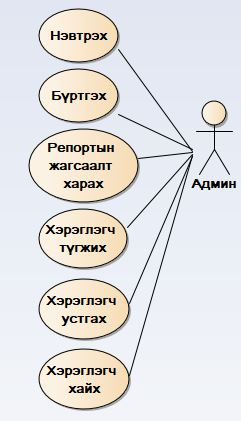
\includegraphics[width=\textwidth]{adminUseCase}
	\subsection{Хэрэглэгчийн юзкейс диаграм}
     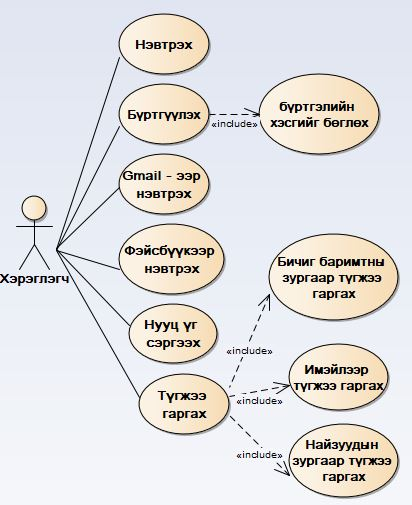
\includegraphics[width=\textwidth]{userUseCase}
     
     	\section{Интерфэйс}
     	\subsection{Нэвтрэх хэсгийн интерфэйс}
     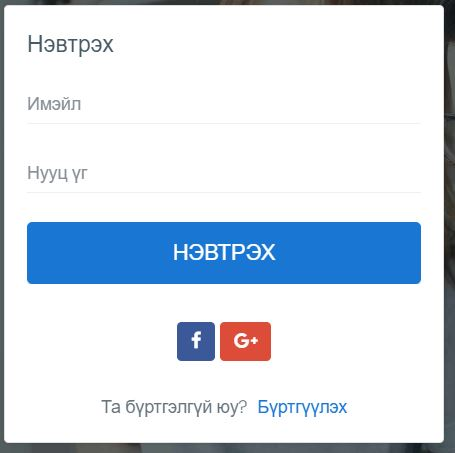
\includegraphics[width=\textwidth]{login}
     \subsection{Бүртгүүлэх хэсгийн интерфэйс}
     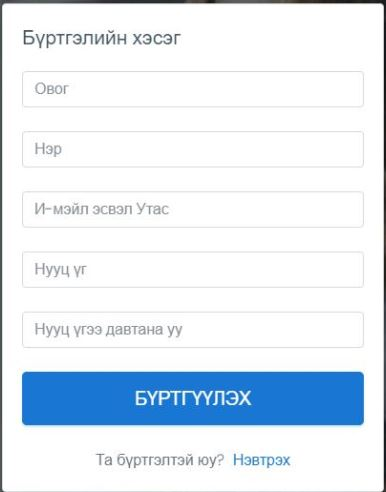
\includegraphics[width=\textwidth]{delgets}
     \subsection{Админы интерфэйс}
     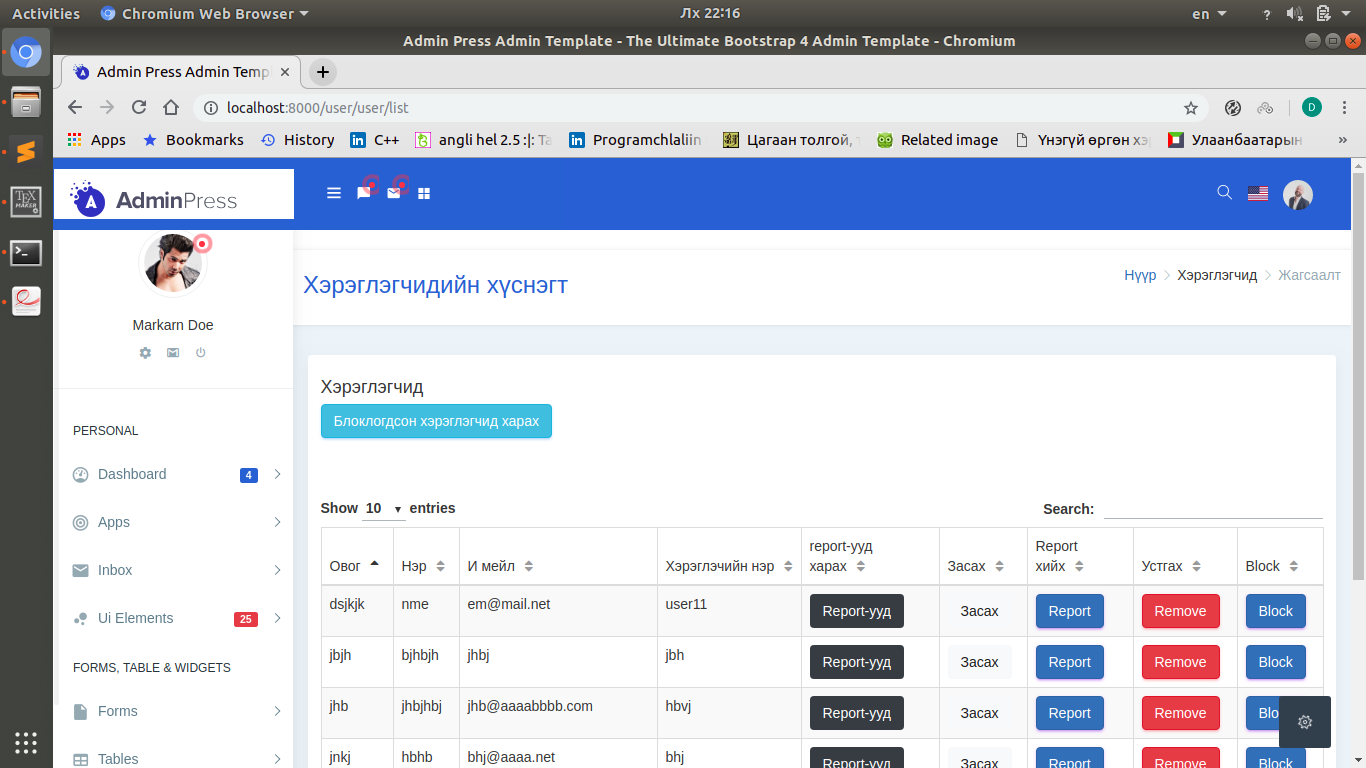
\includegraphics[width=\textwidth]{delgets1}
      \subsection{Репортлох интерфэйс}
     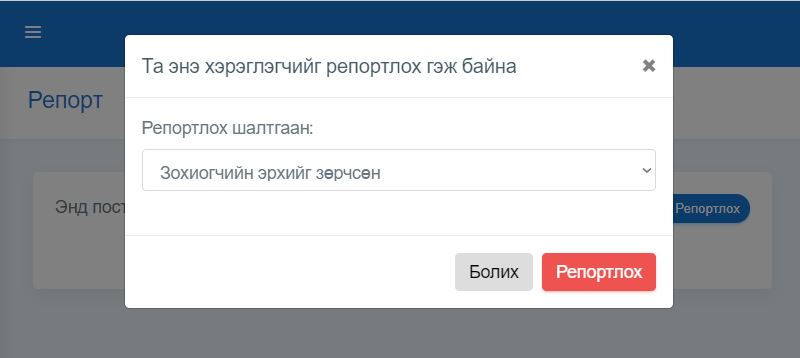
\includegraphics[width=\textwidth]{delgets2}
     \subsection{ Блоклох интерфэйс}
     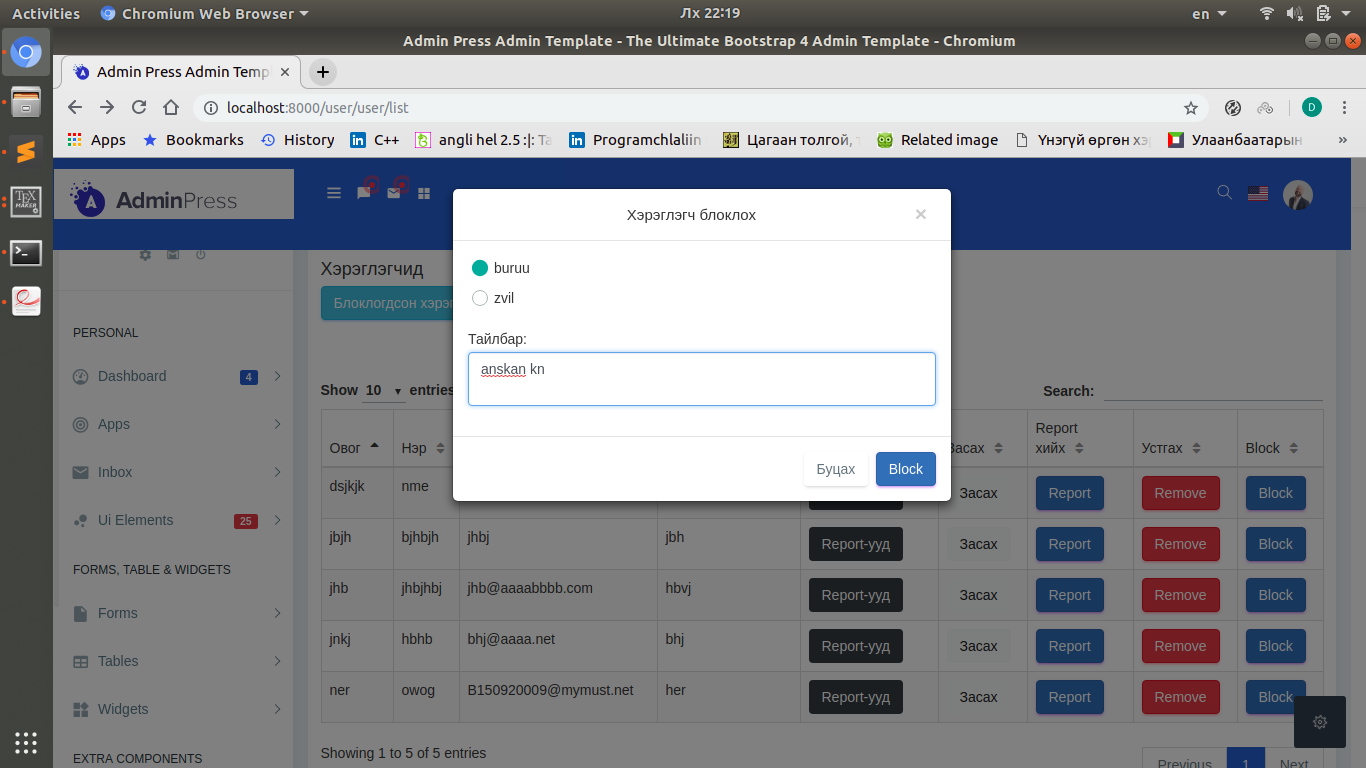
\includegraphics[width=\textwidth]{delgets3}
     \subsection{ Нууц үг сэргээх интерфэйс}
     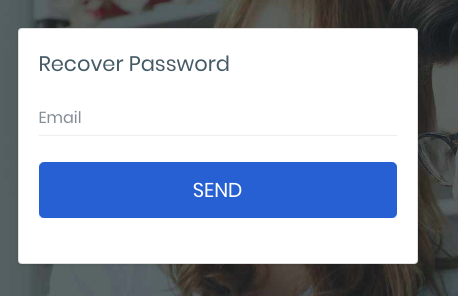
\includegraphics[width=190pt, height=150pt]{forget1}
     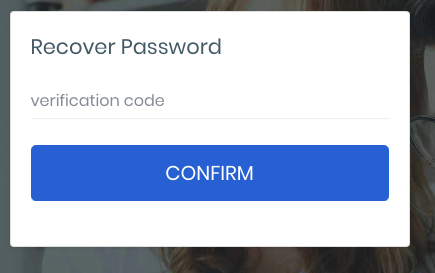
\includegraphics[width=190pt, height=150pt]{forget2}\newline \break
     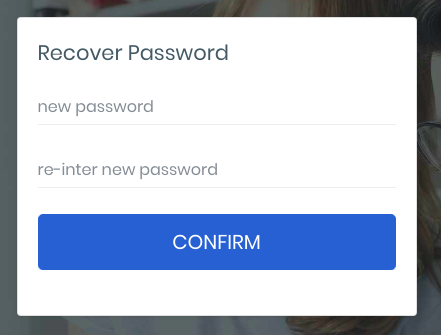
\includegraphics[width=190pt, height=150pt]{forget3}
     
     \section{Бизнесс процессын диаграм}
     	\subsection{Хэрэглэгчийн блок гаргах бизнес процесс }
     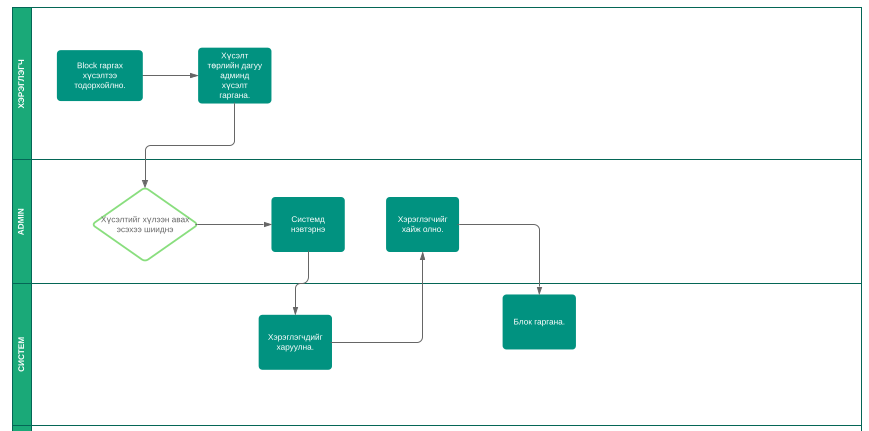
\includegraphics[width=\textwidth]{BP}
     	
     	\section{Үйл ажиллагааны диаграм}
     	\subsection{Бүртгүүлэх үйл ажиллагааны диаграм}
     	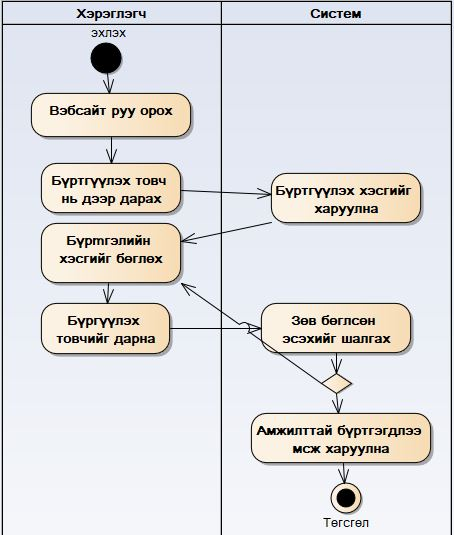
\includegraphics[width=\textwidth]{regActivity}
     	\subsection{Нэвтрэх үйл ажиллагааны диаграм}
     	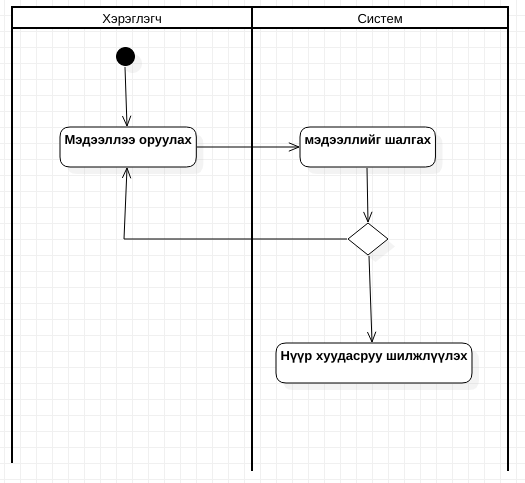
\includegraphics[width=\textwidth]{loginActivity}
     	\subsection{Хэрэглэгч түгжих үйл ажиллагааны диаграм}
     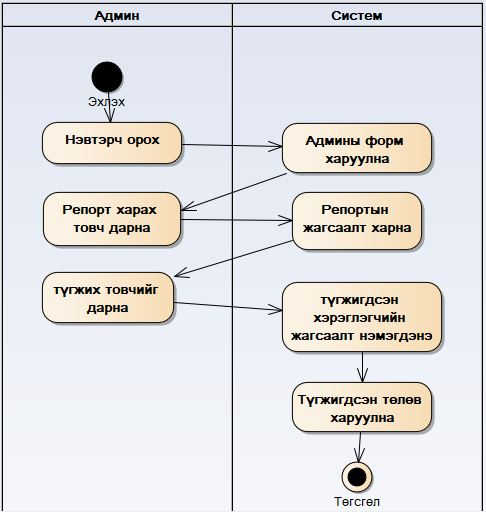
\includegraphics[width=\textwidth]{tugjihActivity}
     \section{Хэрэглэгч түгжээгээ тайлах үйл ажиллагааны диаграм}
     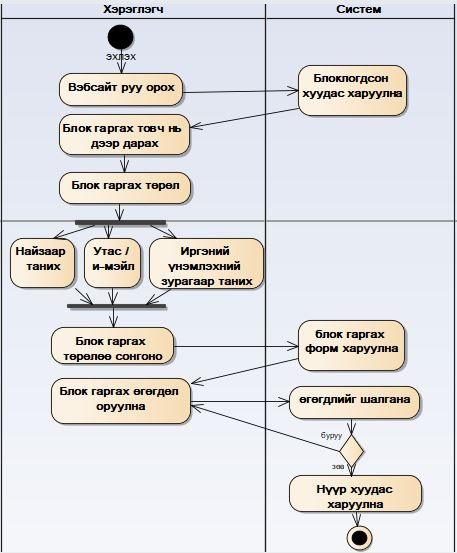
\includegraphics[width=\textwidth]{unblockActivity}
     
     \section{Обьектын холбоосын диаграмм ( ERD )}
     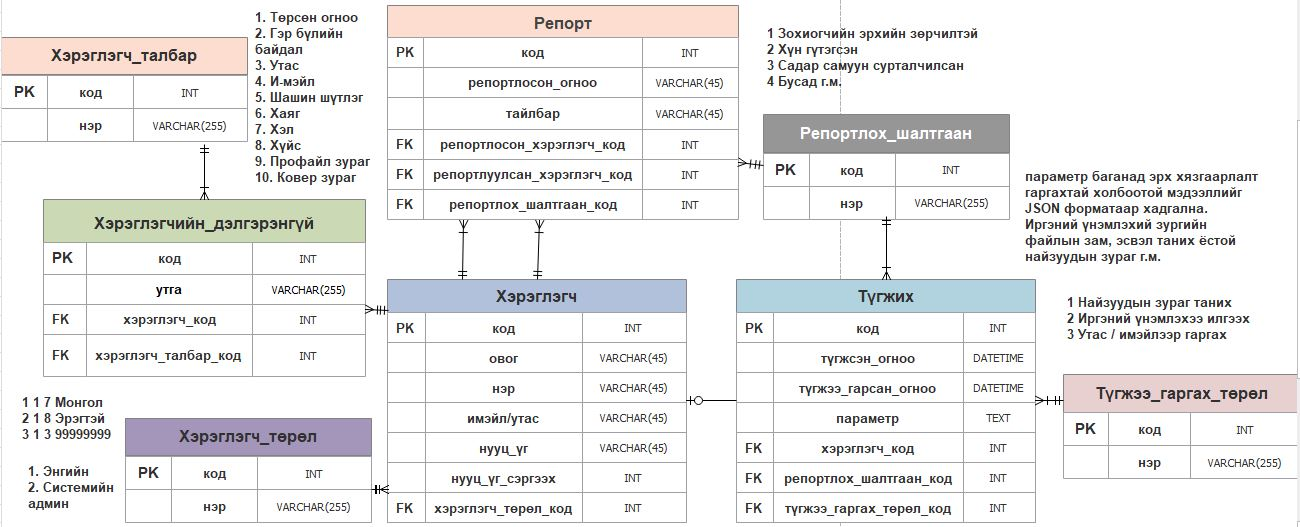
\includegraphics[width=\textwidth]{ERDagram}
     
      \section{Класс диаграм ( Class diagram )}
     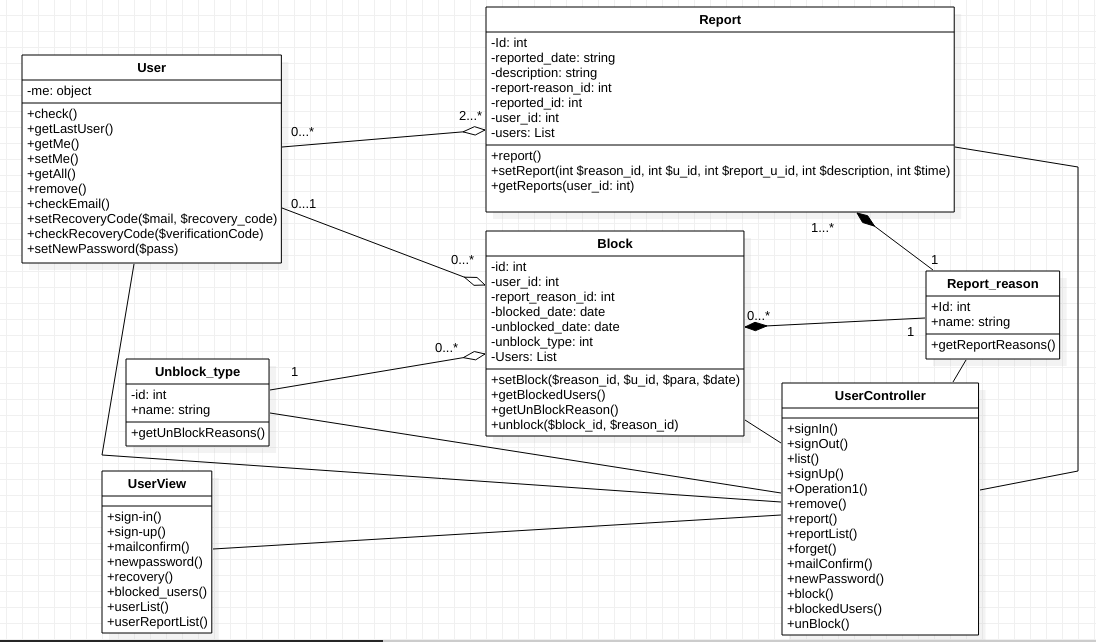
\includegraphics[width=\textwidth]{classdiagram}
     
     \section{Дараалалын диаграмм( Sequence diagram )}
     \subsection{Хэрэглэгч нэвтрэх}
     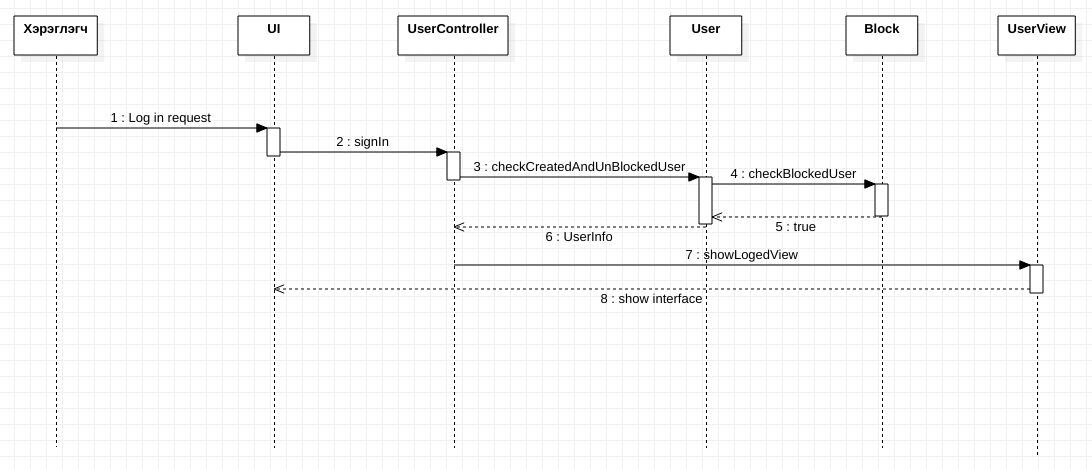
\includegraphics[width=\textwidth]{loginAccess}
     \subsection{Хэрэглэгч блоклох}
     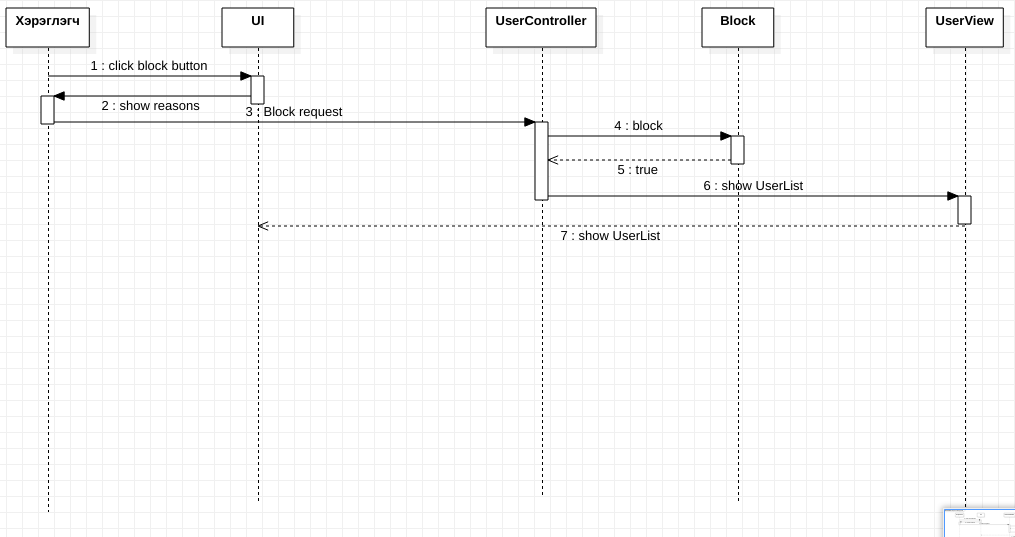
\includegraphics[width=\textwidth]{block}
     \subsection{Хэрэглэгч репортлох}
     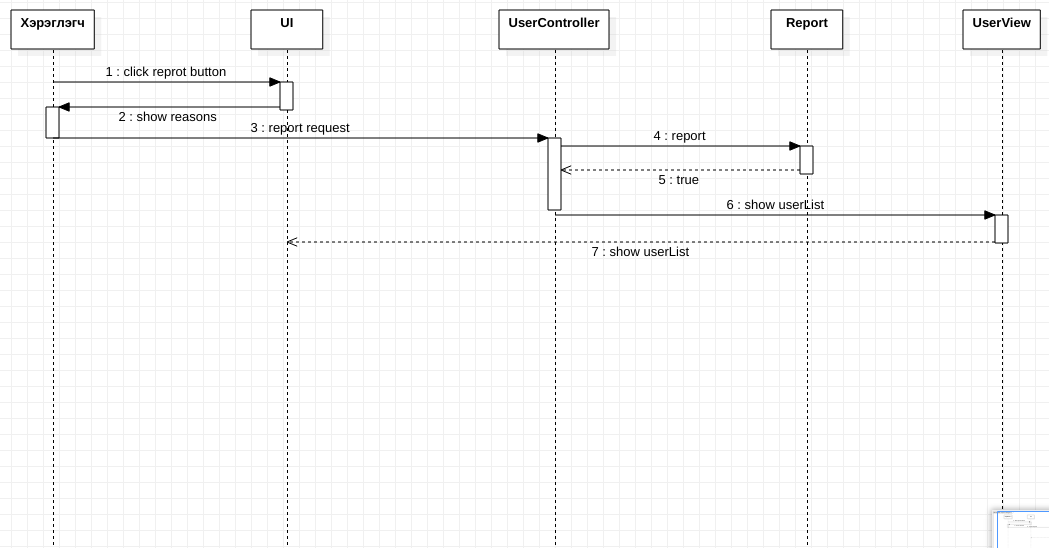
\includegraphics[width=\textwidth]{reportSequence}
     \subsection{Хэрэглэгч блокоос гаргах}
     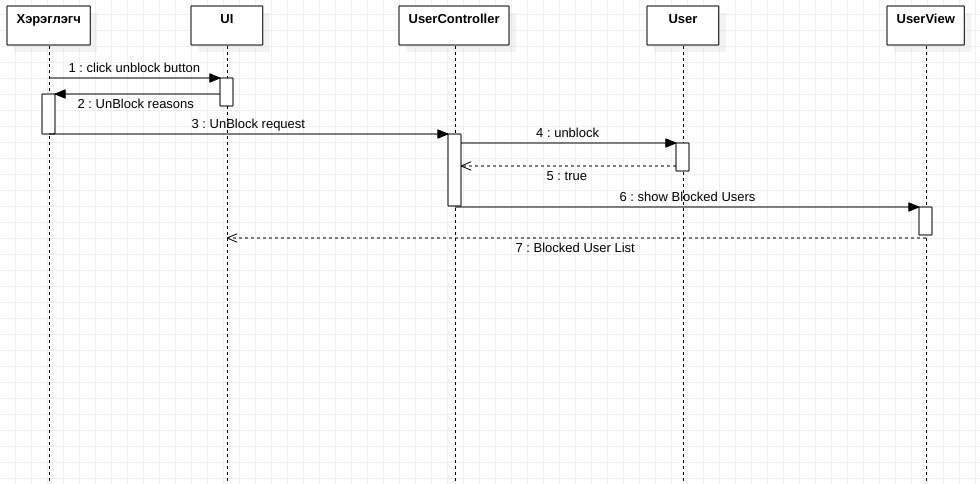
\includegraphics[width=\textwidth]{unBlock}
     
      \section{Төлөвийн диаграм }
     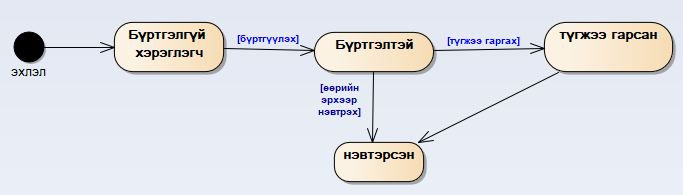
\includegraphics[width=\textwidth]{statechartDiagram}
     
     \section{ Тестын зохиомж }
      \subsection{UserController классын block функцын тест }
     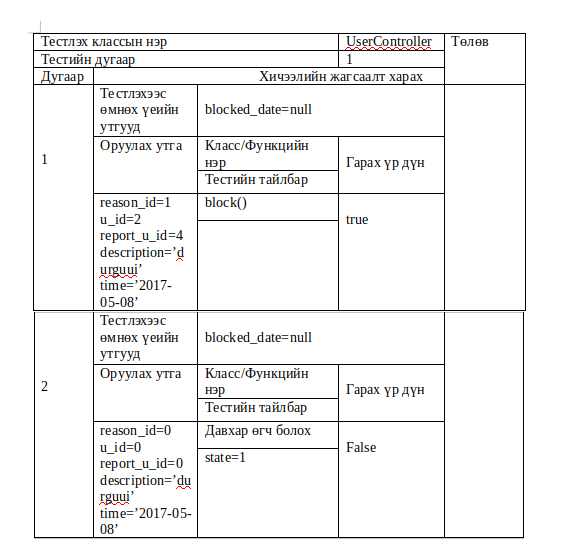
\includegraphics[width=\textwidth]{test1}
      \subsection{User классын report функцын тест}
     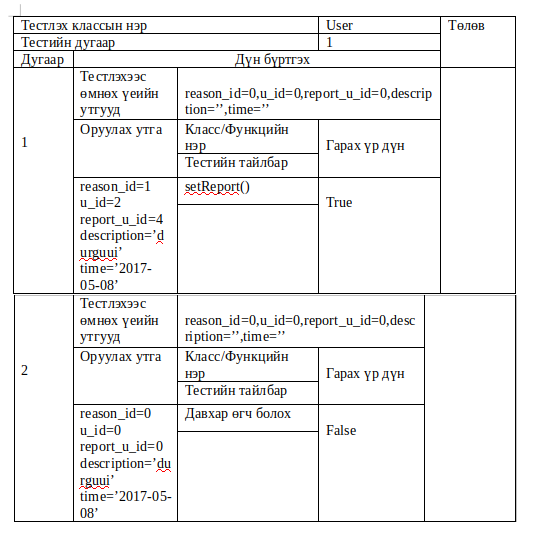
\includegraphics[width=\textwidth]{test2}
     
     
\end{document}